% Capítulo 4
\chapter{Quick Sort}
A função partition necessária para o funcionamento do quick-sort foi implementada pegando como pivô o último elemento da entrada para todos os casos.
\newpage
\section{Gráficos}
\subsection{Melhor caso}
O gráfico abaixo representa o tempo de execução do melhor caso do quick-sort em função do tamanho da entrada. Como entrada para gerar o gráfico, foram utilizados 91 vetores já ordenados, porém, com as posições do meio trocadas com a última posição para forçar o melhor caso. Pela análise do gráfico podemos notar que o algoritmo no melhor caso, desconsiderando a variação de tempo gerada por processos concorrentes no momento da execução do programa, pertence a O(n*log(n)).
\begin{figure}[h]
    \centering
    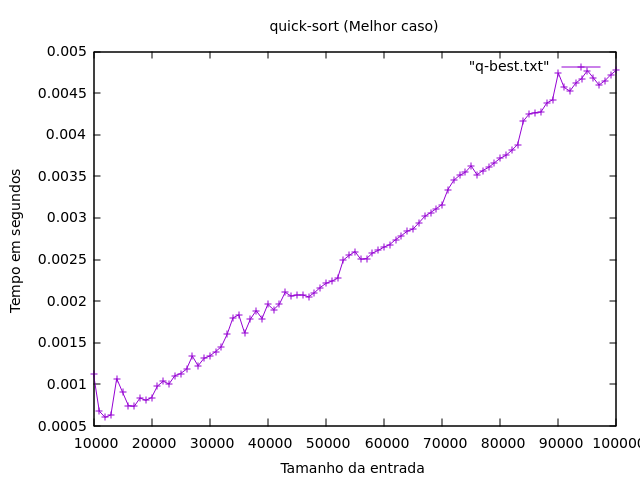
\includegraphics[width=1\linewidth]{Imagens/q-best.png}
\end{figure}

\newpage

\subsection{Pior caso}
O gráfico abaixo representa o tempo de execução do pior caso do quick-sort em função do tamanho da entrada. Como entrada para gerar o gráfico, foram utilizados 91 vetores já ordenados em ordem crescente. Pela análise do gráfico podemos notar que o algoritmo no pior caso, desconsiderando a variação de tempo gerada por processos concorrentes no momento da execução do programa, é quadrático. Tw(n) pertence a O(n²).
\begin{figure}[h]
    \centering
    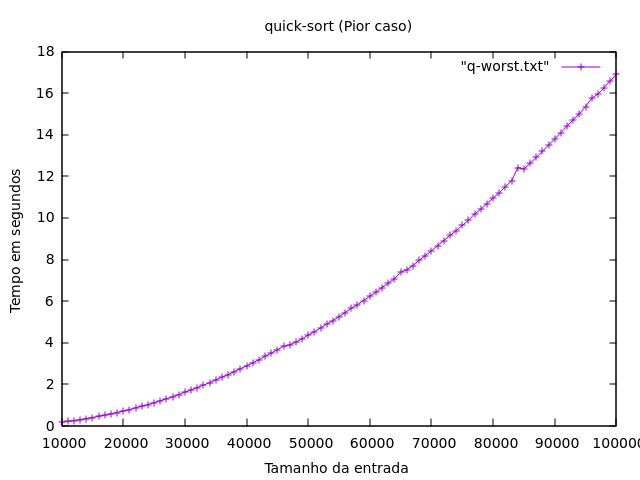
\includegraphics[width=1\linewidth]{Imagens/q-worst.png}
\end{figure}

\newpage

\subsection{Caso médio}
O gráfico abaixo representa o tempo de execução esperado do quick-sort em função do tamanho da entrada. Como entrada para gerar o gráfico, foram utilizados 91 vetores de tamanho n, preenchidos com números de 0 até n gerados aleatoriamente. Pela análise do gráfico podemos notar que o algoritmo no caso médio, desconsiderando a variação de tempo gerada por processos concorrentes no momento da execução do programa, pertence a O(n*log(n)).
\begin{figure}[h]
    \centering
    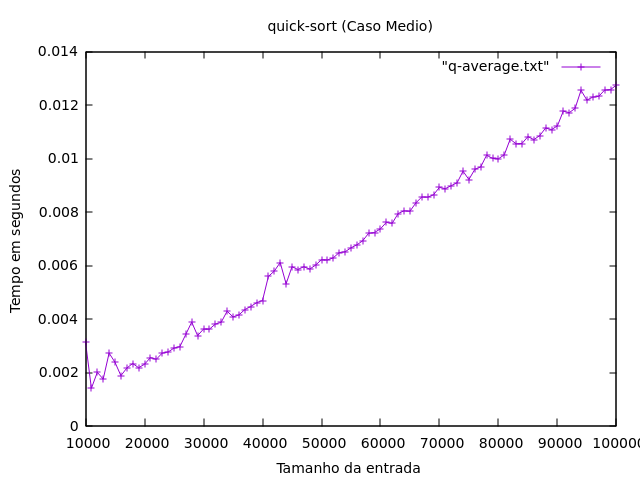
\includegraphics[width=1\linewidth]{Imagens/q-average.png}
\end{figure}

\newpage

\subsection{Comparação dos gráficos}
No gráfico abaixo podemos ver a comparação entre o caso médio, o melhor e o pior caso do algoritmo. É possível perceber que o tempo esperado e o melhor caso tem tempo muito inferior ao tempo do pior caso.
\begin{figure}[h]
    \centering
    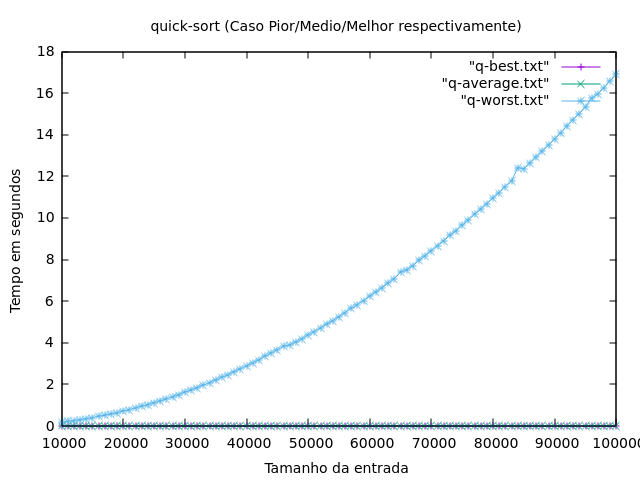
\includegraphics[width=1\linewidth]{Imagens/q-baw.png}
\end{figure}

\newpage

\section{Análise analítica do tempo de execução}
\subsection{Algoritmo}
\begin{figure}[h]
    \centering
    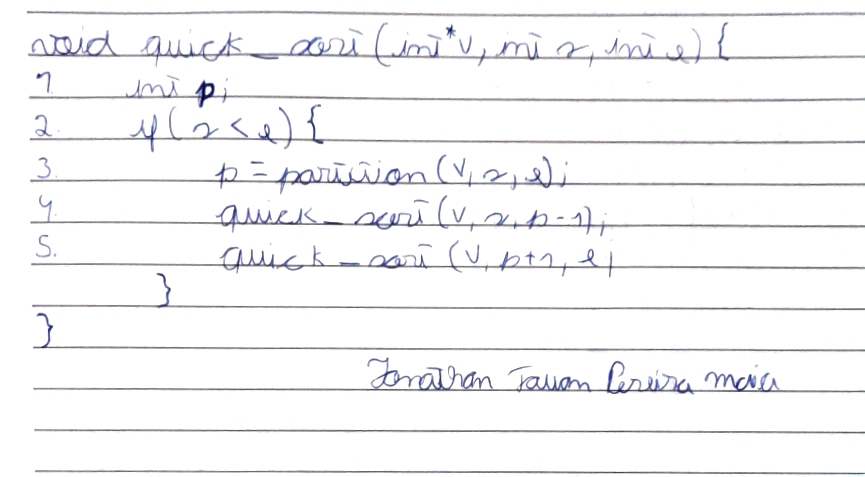
\includegraphics[width=0.76\linewidth]{Imagens/quick.jpg}
\end{figure}

\newpage

\subsubsection{Melhor caso}
A análise analítica do tempo de execução do quick-sort no seu melhor caso, que se dá quando o vetor já está ordenado, porém, com o elemento da posição do meio invertido com o último elemento do vetor, e temos como pivô a última posição, permitiu perceber que seu tempo de execução será (n*log (n)).
\begin{figure}[h]
    \centering
    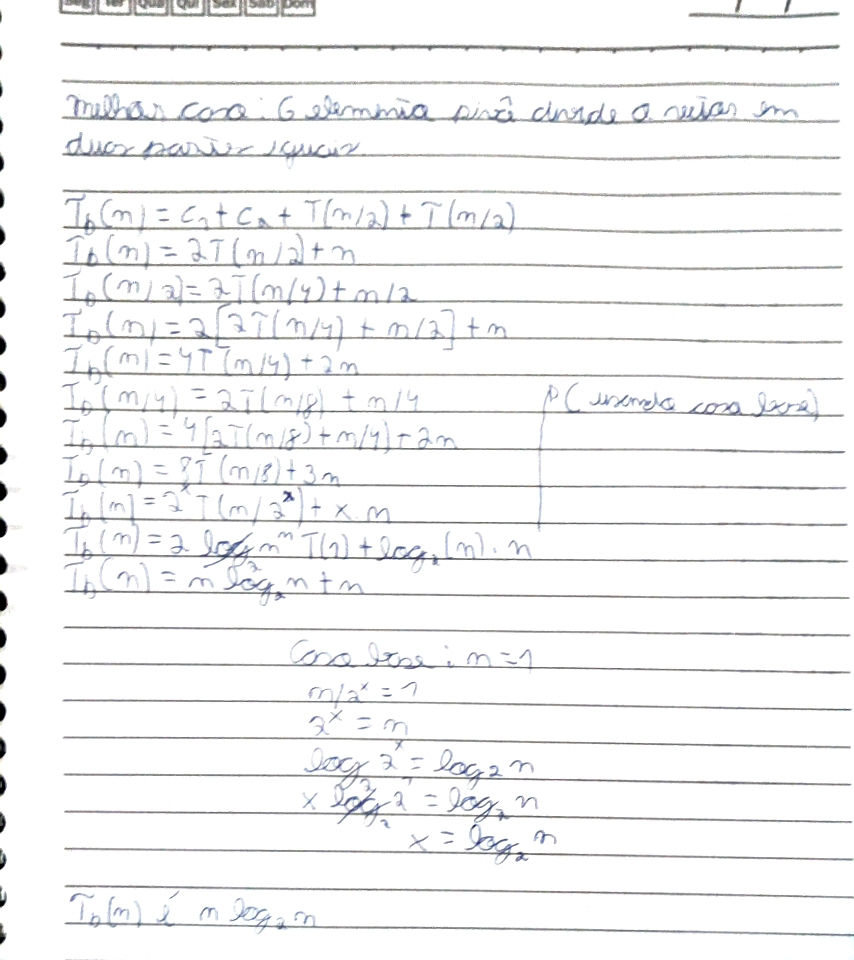
\includegraphics[width=0.76\linewidth]{Imagens/melhor-quick.jpg}
\end{figure}

\newpage

\subsubsection{Pior caso}
A análise analítica do tempo de execução do quick-sort no seu pior caso, que se dá quando o vetor já está ordenado, e pegamos o pivô também como o último elemento do vetor, permitiu perceber que seu tempo de execução será quadrático,  f(n) = an² +
bn + c.
\begin{figure}[h]
    \centering
    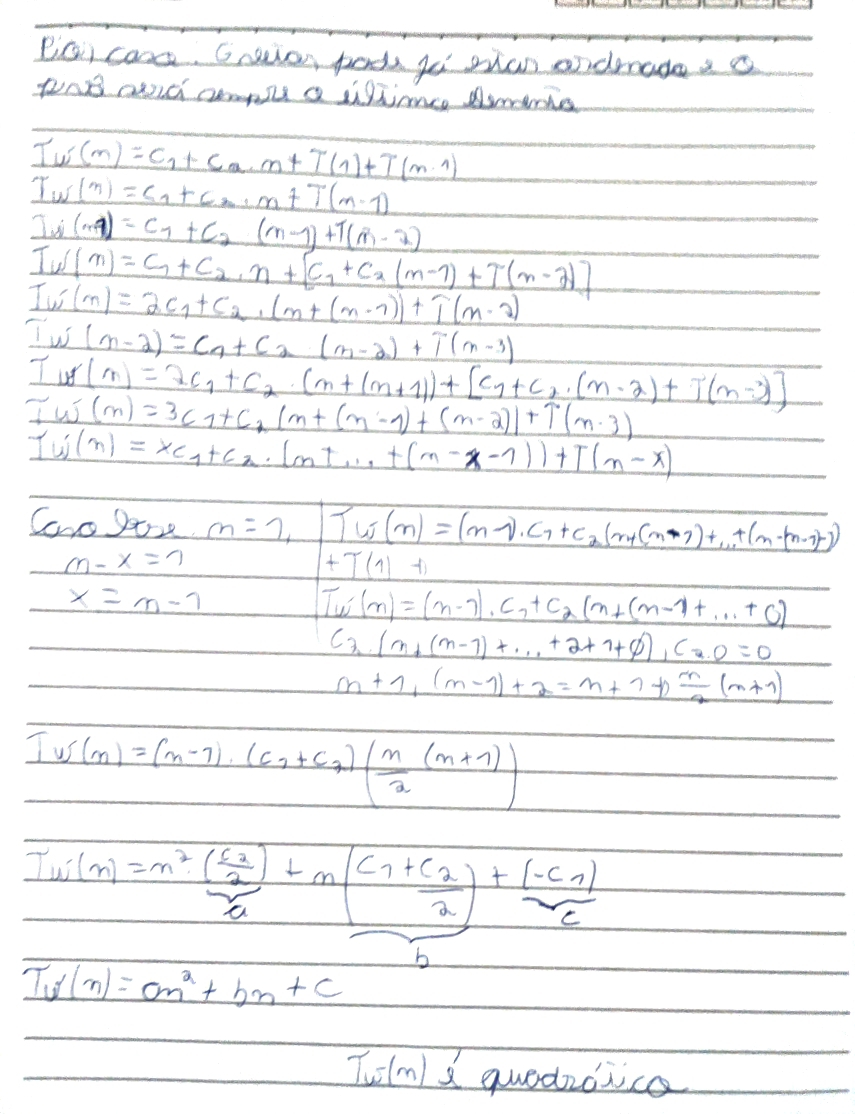
\includegraphics[width=0.76\linewidth]{Imagens/pior-quick.jpg}
\end{figure}